
\subsection{Evaluation of the convective terms}

The discretized convection--diffusion equations requires the values of certain variables at points different from the nodes. In this section several methods to compute $\phi$ at faces are given. The values of $\rho$ and $\Gamma$ will be assumed to be known at the nodal points. East face will be taken as reference for simplicity. The generalization to the remaining faces is straightforward. 

\subsubsection{Upwind--Difference Scheme (UDS)}

Incompressible flows and gases at low Mach number are more influenced by upstream conditions than downstream conditions. Let $(\vb{v} \vdot \vb{n})_e$ denote the value of the dot product $\vb{v} \vdot \vb{n}$ at east face $\cs{Pe}$. If $(\vb{v} \vdot \vb{n})_e > 0$, fluid flows from node $P$ to node $E$, hence $P$ is the upstream node and $E$ is the downstream node. Conversely, if $(\vb{v} \vdot \vb{n})_e < 0$, nodes interchange their roles as fluid flows from node $E$ to node $P$. This situation is pictured in figures \ref{fig:uds_positive_dot_product} and \ref{fig:uds_negative_dot_product}.

\begin{figure}[h]
	\centering
	\begin{minipage}{.5\textwidth}
		\centering
		\begin{tikzpicture}
			% Fill
			\fill[black!20!white] (0,0) rectangle (6,2);
			% Nodes
			\filldraw[greenNode] (1.5,1) circle (2.5pt);
			\node[greenNode, yshift=0.3cm] at (1.5,1) {$P$};
			\filldraw[greenNode] (4.5,1) circle (2.5pt);
			\node[greenNode, yshift=0.3cm] at (4.5,1) {$E$};
			% Vectors
			\draw[->, thick, blue!70!white, yshift=+0.5mm] (3,1) -- node[above]{$\vb{n}$} ++(1,0);
			\draw[->, thick, red!70!white, yshift=-0.5mm] (3,1) -- node[below]{$\vb{v}$} ++(0.75,0);
			% Control volumes
			\draw[thick] (0,0) rectangle (6,2);
			\draw[thick] (3,0) -- ++(0,2);
			\node[circle, inner sep=0pt, outer sep=0pt, black, yshift=0.5cm, fill=black!20!white] at (3,0) {$\cs{Pe}$};
		\end{tikzpicture}
		\captionsetup{width=0.9\textwidth}
		\caption{Since $(\vb{v} \vdot \vb{n})_e > 0$ fluid flows from node $P$ (upstream node) to node $E$ (downstream node).}
		\label{fig:uds_positive_dot_product}
	\end{minipage}%
	\begin{minipage}{.5\textwidth}
		\centering
		\begin{tikzpicture}
			% Fill
			\fill[black!20!white] (0,0) rectangle (6,2);
			% Nodes
			\filldraw[greenNode] (1.5,1) circle (2.5pt);
			\node[greenNode, yshift=0.3cm] at (1.5,1) {$P$};
			\filldraw[greenNode] (4.5,1) circle (2.5pt);
			\node[greenNode, yshift=0.3cm] at (4.5,1) {$E$};			
			% Vectors
			\draw[->, thick, blue!70!white] (3,1) -- node[above]{$\vb{n}$} ++(1,0);
			\draw[->, thick, red!70!white] (3,1) -- node[above]{$\vb{v}$} ++(-0.75,0);			
			% Control volumes
			\draw[thick] (0,0) rectangle (6,2);
			\draw[thick] (3,0) -- ++(0,2);
			\node[circle, inner sep=0pt, outer sep=0pt, black, yshift=0.5cm, fill=black!20!white] at (3,0) {$\cs{Pe}$};
		\end{tikzpicture}
		\captionsetup{width=0.9\textwidth}
		\caption{Since $(\vb{v} \vdot \vb{n})_e < 0$ fluid flows from node $E$ (upstream node) to node $P$ (downstream node).}
		\label{fig:uds_negative_dot_product}
	\end{minipage}
\end{figure}

\noindent
If $(\vb{v} \vdot \vb{n})_e = 0$, it implies $\vb{v}_e$ lies in the orthogonal subspace to the vector space generated by $\vb{n}$. As a result, given the approximations taken, there is no fluid flow through face $\cs{Pe}$.

The Upwind--Difference Scheme assigns $\phi_e$ the value of $\phi$ at the upstream node, that is,
\begin{equation}
	\phi_e^\text{UDS} = 
	\left\{
	\begin{aligned}
		&\phi_P & &\text{if } (\vb{v} \vdot \vb{n})_e > 0 \\
		&\phi_E & &\text{if } (\vb{v} \vdot \vb{n})_e < 0 \\
	\end{aligned}
	\right.
\end{equation}
This can be expressed in a more compact form as follows
\begin{equation}
	\dot{m}_e ( \phi_e - \phi_P ) = 
	\frac{\dot{m}_e - \abs{\dot{m}_e}}{2} ( \phi_E - \phi_P )
\end{equation}
since the approximation to compute $\dot{m}_e$ is related to $(\vb{v} \vdot \vb{n})_e$ through the relation $\dot{m}_e = (\vb{v} \vdot \vb{n})_e S_{Pe}$. The scheme is shown in figures \ref{fig:uds_upstream_node_P} and \ref{fig:uds_upstream_node_E}.

\begin{figure}[h]
	\centering
	\begin{minipage}{.5\textwidth}
		\centering
		\begin{tikzpicture}
			% Ground
			\draw[thick] (0,0) -- ++(6,0);
			% Point P
			\filldraw[black] (0.5,0) circle (2pt);
			\draw[dashed] (0.5,0) -- ++(0,1.5);
			\node[black, yshift=-0.5cm] at (0.5,0) {$P$};
			\filldraw[blue!70!white] (0.5,1.5) circle (2pt);
			\node[blue, yshift=0.5cm] at (0.5,1.5) {$\phi_P$};
			% Point e
			\filldraw[black] (2.5,0) circle (2pt);
			\draw[dashed] (2.5,0) -- ++(0,1.5);
			\node[black, yshift=-0.5cm] at (2.5,0) {$e$};
			\filldraw[blue!70!white] (2.5,1.5) circle (2pt);
			\node[blue, yshift=0.5cm] at (2.5,1.5) {$\phi_e$}; 
			% Point E
			\filldraw[black] (5.5,0) circle (2pt);
			\draw[dashed] (5.5,0) -- ++(0,3);
			\node[black, yshift=-0.5cm] at (5.5,0) {$E$};
			\filldraw[blue!70!white] (5.5,3.0) circle (2pt);
			\node[blue, yshift=0.5cm] at (5.5,3.0) {$\phi_E$};
			% Blue line
			\begin{scope}[very thick,decoration={
					markings,
					mark=at position 0.5 with {\arrow{>}}}
				] 
				\draw[thick, blue!70!white, postaction={decorate}] (0.5,1.5) -- ++(2,0);
			\end{scope}
			% Mass flow
			\draw[->, red, thick] (1.75,0.75) -- ++(1.5,0) node[above]{$\dot{m}_e > 0$};
		\end{tikzpicture}
		\captionsetup{width=0.9\textwidth}
		\caption{UDS when $(\vb{v} \vdot \vb{n})_e > 0$.}
		\label{fig:uds_upstream_node_P}
	\end{minipage}%
	\begin{minipage}{.5\textwidth}
		\centering
		\begin{tikzpicture}
			% Ground
			\draw[thick] (0,0) -- ++(6,0);
			% Point P
			\filldraw[black] (0.5,0) circle (2pt);
			\draw[dashed] (0.5,0) -- ++(0,1.5);
			\node[black, yshift=-0.5cm] at (0.5,0) {$P$};
			\filldraw[blue!70!white] (0.5,1.5) circle (2pt);
			\node[blue, yshift=0.5cm] at (0.5,1.5) {$\phi_P$};
			% Point e
			\filldraw[black] (2.5,0) circle (2pt);
			\draw[dashed] (2.5,0) -- ++(0,3);
			\node[black, yshift=-0.5cm] at (2.5,0) {$e$};
			\filldraw[blue!70!white] (2.5,3) circle (2pt);
			\node[blue, yshift=0.5cm] at (2.5,3.0) {$\phi_e$}; 
			% Point E
			\filldraw[black] (5.5,0) circle (2pt);
			\draw[dashed] (5.5,0) -- ++(0,3);
			\node[black, yshift=-0.5cm] at (5.5,0) {$E$};
			\filldraw[blue!70!white] (5.5,3) circle (2pt);
			\node[blue, yshift=0.5cm] at (5.5,3.0) {$\phi_e$}; 
			% Blue line
			\begin{scope}[very thick,decoration={
					markings,
					mark=at position 0.5 with {\arrow{<}}}
				] 
				\draw[thick, blue!70!white, postaction={decorate}] (2.5,3.0) -- ++(3,0);
			\end{scope}
			% Mass flow
			\draw[->, red, thick] (1.75,0.75) -- ++(1.5,0) node[above]{$\dot{m}_e < 0$};
		\end{tikzpicture}
		\captionsetup{width=0.9\textwidth}
		\caption{UDS when $(\vb{v} \vdot \vb{n})_e < 0$.}
		\label{fig:uds_upstream_node_E}
	\end{minipage}
\end{figure}


UDS is a stable scheme, however it suffers from numerical diffusion. Indeed, assuming the upstream node is $P$, expanding $\phi$ about point $x_P$ in its Taylor expansion up to $2^\text{nd}$ degree and using Lagrange's remainder,
\begin{equation} \label{eq:UDS_taylor_polynomial_P}
	\phi_e = 
	\phi_P + \left(\pdv{\phi}{x}\right)_P d_{Pe} + 
	\left(\pdv[2]{\phi}{x}\right)_{\xi_1} \frac{d_{Pe}^2}{2}
\end{equation}
it is apparent that UDS retains the first term on the left--hand side of \eqref{eq:UDS_taylor_polynomial_P}. As a consequence, the highest order term of the error is $(\partial_x \phi)_P d_{Pe}$, which is proportional to the distance between $P$ and the face $\cs{Pe}$. This term resembles to a diffusion flux given, for instance, by Fourier's or Fick's laws of diffusion. The same result is obtained when $E$ is the upstream node,
\begin{equation}
	\phi_e = 
	\phi_E - \left(\pdv{\phi}{x}\right)_E d_{Ee} + \left(\pdv[2]{\phi}{x}\right)_{\xi_2} \frac{d_{Ee}^2}{2}
\end{equation}
whence it can be deduced that the error is bounded by $\max\{ \abs{(\partial_x \phi)_E d_{Pe}}, \abs{(\partial_x \phi)_E d_{Ee}}\}$. The numerical diffusion issue is magnified in multidimensional problems, where peaks of rapid variation can be obtained, hence very fine grids are required. 

\subsubsection{Central--Difference Scheme (CDS)}

The Central--Difference Scheme assumes a linear distribution for $\phi$ as illustrated in figure \ref{fig:central_difference_scheme},
\begin{figure}[h]
	\centering
	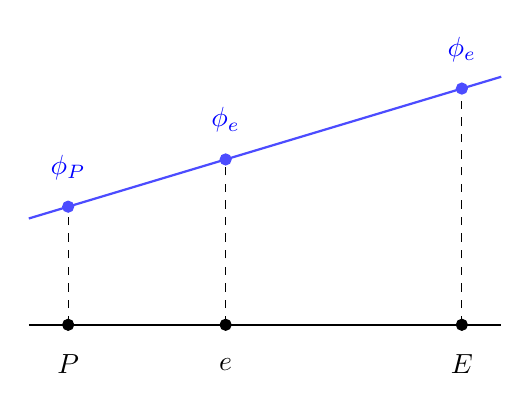
\begin{tikzpicture}
		% Ground
		\draw[thick] (0,0) -- ++(6,0);
		% Point P
		\filldraw[black] (0.5,0) circle (2pt);
		\draw[dashed] (0.5,0) -- ++(0,1.5);
		\node[black, yshift=-0.5cm] at (0.5,0) {$P$};
		\filldraw[blue!70!white] (0.5,1.5) circle (2pt);
		\node[blue, yshift=0.5cm] at (0.5,1.5) {$\phi_P$};
		% Point e
		\filldraw[black] (2.5,0) circle (2pt);
		\draw[dashed] (2.5,0) -- ++(0,{1.5+3/5});
		\node[black, yshift=-0.5cm] at (2.5,0) {$e$};
		\filldraw[blue!70!white] (2.5,{1.5+3/5}) circle (2pt);
		\node[blue, yshift=0.5cm] at (2.5,{1.5+3/5}) {$\phi_e$}; 
		% Point E
		\filldraw[black] (5.5,0) circle (2pt);
		\draw[dashed] (5.5,0) -- ++(0,3);
		\node[black, yshift=-0.5cm] at (5.5,0) {$E$};
		\filldraw[blue!70!white] (5.5,3) circle (2pt);
		\node[blue, yshift=0.5cm] at (5.5,3.0) {$\phi_e$}; 
		% Blue line
		\draw[thick, blue!70!white] (0,{1.5-1.5/10}) -- (6,{1.5+1.5*5.5/5});
	\end{tikzpicture}
	\caption{Central Difference Scheme (CDS).}
	\label{fig:central_difference_scheme}
\end{figure}

\noindent
Thereby $\phi_e$ can be obtained interpolating between $\phi_P$ and $\phi_E$,
\begin{equation}
	\phi_e - \phi_P = f_e \left( \phi_E - \phi_P \right), \quad f_e = \frac{d_{Pe}}{d_{PE}}
\end{equation}
This yields a $2^{\text{nd}}$ order approximation for $\phi_e$ if $d_{Pe} = d_{Ee}$. In effect, applying Taylor's theorem about point $x_e$,
\begin{equation} \label{eq:cds_taylor_expansion}
	\phi_P = 
	\phi_e 
	- \left(\pdv{\phi}{x}\right)_e d_{Pe} 
	+ \frac{1}{2} \left(\pdv[2]{\phi}{x}\right)_e d_{Pe}^2 
	+ \frac{1}{6} \left(\pdv[3]{\phi}{x}\right)_{\xi_1} d_{Pe}^3
\end{equation}
The $2^\text{nd}$ order approximation of $(\partial_x \phi)_e$ is given by
\begin{equation} \label{eq:cds_derivative_approximation}
	\left(\pdv{\phi}{x}\right)_e = 
	\frac{\phi_E - \phi_P}{d_{PE}} - \left(\pdv[3]{\phi}{x}\right)_{\xi_2} \frac{d_{PE}^2}{3!} = 	
	\frac{\phi_E - \phi_P}{d_{PE}} - \left(\pdv[3]{\phi}{x}\right)_{\xi_2} \frac{(d_{Pe} + d_{Ee})^2}{3!}
\end{equation}
Introducing \eqref{eq:cds_derivative_approximation} in \eqref{eq:cds_taylor_expansion} and imposing $d_{Pe} = d_{Ee}$, 
\begin{equation} \label{eq:cds_error_terms}
	\phi_e - \phi_P = 
	\frac{d_{Pe}}{d_{PE}} (\phi_E - \phi_P) - 
	\left( \pdv[2]{\phi}{x} \right)_e \frac{d_{Pe}^2}{2} -
	\left\{ 
	\left( \pdv[3]{\phi}{x} \right)_{\xi_1} + 4 \left( \pdv[3]{\phi}{x} \right)_{\xi_2}
	\right\} 
	\frac{d_{Pe}^3}{6}
\end{equation}
As CDS retains the first term on the left--hand side of \eqref{eq:cds_error_terms}, the highest order term of the error is $\frac{1}{2} (\partial_x^2 \phi)_e d_{Pe}^2$, proving that CDS provides a $2^\text{nd}$ order approximation of $\phi_e$ when $d_{Pe} = d_{Ee}$. Nonetheless, this scheme is prone to stability problems producing oscillatory outputs since the approximation is of order higher than $1$.

\subsubsection{Second--order Upwind Linear Extrapolation (SUDS)}

As stated previously, incompressible flows and fluids at low Mach number are more influenced by upstream condition than downstream conditions. In order to account for this fact and to ease the study, some notation is introduced. Located at the face separating two control volumes, $f$ refers to the face, $D$ is the downstream node, $C$ is the first upstream node and $U$ is the most upstream node. Some books may use $U$ and $UU$ instead of $C$ and $U$, respectively.

The Second--order Upwind Linear Extrapolation scheme takes profit of this idea since it extrapolates $\phi_e$ using a straight line between the values of $\phi$ at nodes $C$ and $U$. The two possible situations are pictured in figures \ref{fig:suds_1} and \ref{fig:suds_2}.

\begin{figure}[h]
	\centering
	\begin{minipage}{.5\textwidth}
		\centering
		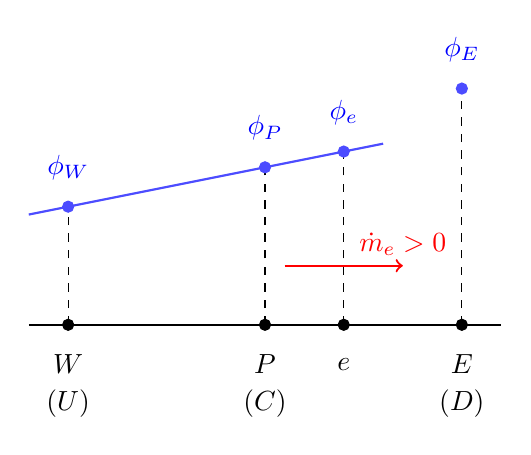
\begin{tikzpicture}
			% Points
			\def\zerox{0.5}
			\def\zeroy{1.5}
			\def\onex{3}
			\def\oney{2}
			\def\twox{5.5}
			\def\twoy{3}
			\def\coefa{1.5}
			\def\coefb{0.2}
			\def\coefc{0.04}
			% Ground
			\draw[thick] (0,0) -- ++(6,0);
			% Point W
			\filldraw[black] (\zerox,0) circle (2pt);
			\draw[dashed] (\zerox,0) -- ++(0,\zeroy);
			\node[black, yshift=-0.5cm] at (\zerox,0) {$W$};
			\node[black, yshift=-1cm] at (\zerox,0) {$(U)$};
			\filldraw[blue!70!white] (\zerox,\zeroy) circle (2pt);
			\node[blue, yshift=0.5cm] at (\zerox,\zeroy) {$\phi_W$};
			% Point P
			\filldraw[black] (\onex,0) circle (2pt);
			\draw[dashed] (\onex,0) -- ++(0,\oney);
			\node[black, yshift=-0.5cm] at (\onex,0) {$P$};
			\node[black, yshift=-1cm] at (\onex,0) {$(C)$};
			\filldraw[blue!70!white] (\onex,\oney) circle (2pt);
			\node[blue, yshift=0.5cm] at (\onex,\oney) {$\phi_P$};
			% Point e
			\filldraw[black] ({\onex+1},0) circle (2pt);
			\draw[dashed] ({\onex+1},0) -- ++(0,{1.5+0.5*3.5/2.5});
			\node[black, yshift=-0.5cm] at ({\onex+1},0) {$e$};
			\filldraw[blue!70!white] ({\onex+1},{1.5+0.5*3.5/2.5}) circle (2pt);
			\node[blue, yshift=0.5cm] at ({\onex+1},{1.5+0.5*3.5/2.5}) {$\phi_e$};
			% Point E
			\filldraw[black] (\twox,0) circle (2pt);
			\draw[dashed] (\twox,0) -- ++(0,\twoy);
			\node[black, yshift=-0.5cm] at (\twox,0) {$E$};
			\node[black, yshift=-1cm] at (\twox,0) {$(D)$};
			\filldraw[blue!70!white] (\twox,\twoy) circle (2pt);
			\node[blue, yshift=0.5cm] at (\twox,\twoy) {$\phi_E$}; 
			% Blue line
			\draw[scale=1, domain=0:4.5, smooth, variable=\x, blue!70!white, thick] plot ({\x}, {1.5+0.2*(\x-0.5)});
			% Mass flow
			\draw[->, red, thick] (3.25,0.75) -- ++(1.5,0) node[above]{$\dot{m}_e > 0$};
		\end{tikzpicture}
		\captionsetup{width=0.9\textwidth}
		\caption{SUDS when $(\vb{v} \vdot \vb{n})_e > 0$.}
		\label{fig:suds_1}
	\end{minipage}%
	\begin{minipage}{.5\textwidth}
		\centering
		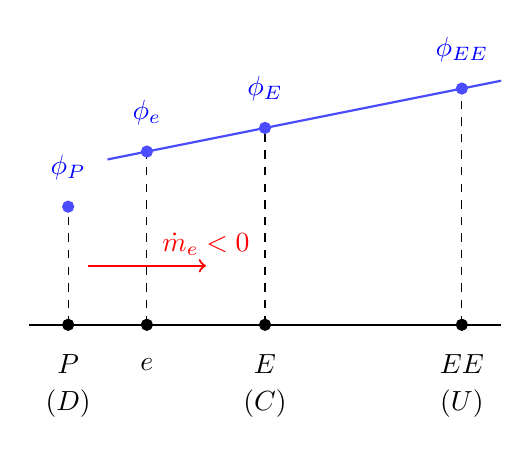
\begin{tikzpicture}
			% Points
			\def\zerox{0.5}
			\def\zeroy{1.5}
			\def\onex{3}
			\def\oney{2.5}
			\def\twox{5.5}
			\def\twoy{3}
			\def\coefa{1.5}
			\def\coefb{0.4}
			\def\coefc{-0.04}
			% Ground
			\draw[thick] (0,0) -- ++(6,0);
			% Point P
			\filldraw[black] (\zerox,0) circle (2pt);
			\draw[dashed] (\zerox,0) -- ++(0,\zeroy);
			\node[black, yshift=-0.5cm] at (\zerox,0) {$P$};
			\node[black, yshift=-1cm] at (\zerox,0) {$(D)$};
			\filldraw[blue!70!white] (\zerox,\zeroy) circle (2pt);
			\node[blue, yshift=0.5cm] at (\zerox,\zeroy) {$\phi_P$};
			% Point e
			\filldraw[black] ({\zerox+1},0) circle (2pt);
			\draw[dashed] ({\zerox+1},0) -- ++(0,{2.5-0.2*1.5});
			\node[black, yshift=-0.5cm] at ({\zerox+1},0) {$e$};
			\filldraw[blue!70!white] ({\zerox+1},{2.5-0.2*1.5}) circle (2pt);
			\node[blue, yshift=0.5cm] at ({\zerox+1},{2.5-0.2*1.5}) {$\phi_e$};
			% Point e
			\filldraw[black] (\onex,0) circle (2pt);
			\draw[dashed] (\onex,0) -- ++(0,\oney);
			\node[black, yshift=-0.5cm] at (\onex,0) {$E$};
			\node[black, yshift=-1cm] at (\onex,0) {$(C)$};
			\filldraw[blue!70!white] (\onex,\oney) circle (2pt);
			\node[blue, yshift=0.5cm] at (\onex,\oney) {$\phi_E$}; 
			% Point ee
			\filldraw[black] (\twox,0) circle (2pt);
			\draw[dashed] (\twox,0) -- ++(0,\twoy);
			\node[black, yshift=-0.5cm] at (\twox,0) {$EE$};
			\node[black, yshift=-1cm] at (\twox,0) {$(U)$};
			\filldraw[blue!70!white] (\twox,\twoy) circle (2pt);
			\node[blue, yshift=0.5cm] at (\twox,\twoy) {$\phi_{EE}$}; 
			% Blue line
			\draw[scale=1, domain=1:6, smooth, variable=\x, blue!70!white, thick] plot ({\x}, {2.5+0.2*(\x-3)});
			% Mass flow
			\draw[->, red, thick] (0.75,0.75) -- ++(1.5,0) node[above]{$\dot{m}_e < 0$};
		\end{tikzpicture}
		\captionsetup{width=0.9\textwidth}
		\caption{SUDS when $(\vb{v} \vdot \vb{n})_e < 0$.}
		\label{fig:suds_2}
	\end{minipage}
\end{figure}

\noindent
On the one hand, when $(\vb{v} \vdot \vb{n})_e > 0$, the line between points $(x_W, \phi_W)$ and $(x_P, \phi_P)$ is given by
\begin{equation}
	\phi(x) = \phi_W + \frac{\phi_P - \phi_W}{d_{PW}} (x - x_W)
\end{equation}
and substituting at $x = x_e$, the formula for $\phi_e$ is obtained:
\begin{equation} \label{eq:suds_1_1}
	\phi_e = 
	\phi(x_e) = 
	\phi_W + \frac{\phi_P - \phi_W}{d_{PW}} (x_e - x_W) = 
	\phi_P + \frac{d_{Pe}}{d_{PW}} (\phi_P - \phi_W) 
\end{equation}
On the other hand, in the case of $(\vb{v} \vdot \vb{n})_e < 0$, the line between points $(x_E, \phi_E)$ and $(x_{EE}, \phi_{EE})$ is
\begin{equation}
	\phi(x) = \phi_E + \frac{\phi_{EE} - \phi_E}{d_{E,EE}} (x - x_E)
\end{equation}
and the approximation of $\phi_e$ is
\begin{equation} \label{eq:suds_2_1}
	\phi_e = 
	\phi(x_e) = 
	\phi_E + \frac{\phi_{EE} - \phi_E}{d_{E,EE}} (x_e - x_E) =
	\phi_E + \frac{d_{Ee}}{d_{E,EE}} (\phi_{EE} - \phi_E)	
\end{equation}
Using the new notation, \eqref{eq:suds_1_1} and \eqref{eq:suds_2_1} are both rewritten in the following manner:
\begin{equation}
	\phi_f - \phi_C = \frac{d_{Cf}}{d_{CU}} (\phi_C - \phi_U)
\end{equation}

In order to prove that SUDS is a second order scheme when a locally uniform mesh is used and $(\vb{v} \vdot \vb{n})_e > 0$, consider the Taylor expansion up to $2^{nd}$ degree of $\phi$ about point $x_W$,
\begin{equation}
	\phi_e = 
	\phi_W + 
	\left( \pdv{\phi}{x} \right)_W d_{We} + 
	\left( \pdv[2]{\phi}{x} \right)_{\xi_1} \frac{d_{We}^2}{2}
\end{equation}
The first derivative of $\phi$ with respect to $x$ can be replaced by its first order approximation, namely,
\begin{equation}
	\left(\pdv{\phi}{x}\right)_W = 
	\frac{\phi_P - \phi_W}{d_{PW}} - \left(\pdv[2]{\phi}{x}\right)_{\xi_2} \frac{d_{PW}}{2}
\end{equation}
thereby,
\begin{align}
	\phi_e 
	&= 
	\phi_W + 
	\frac{d_{We}}{d_{PW}} (\phi_P - \phi_W) + 
	\left( \pdv[2]{\phi}{x} \right)_{\xi_1} \frac{d_{We}^2}{2} - 
	\left( \pdv[2]{\phi}{x} \right)_{\xi_2} \frac{d_{We} d_{PW}}{2} \nonumber \\
	&= 
	\phi_P + 
	\frac{d_{Pe}}{d_{PW}} (\phi_P - \phi_W) + 
	\left( \pdv[2]{\phi}{x} \right)_{\xi_1} \frac{(d_{PW} + d_{Pe})^2}{2} - 
	\left( \pdv[2]{\phi}{x} \right)_{\xi_2} \frac{(d_{PW} + d_{Pe}) d_{PW}}{2}	
	\label{eq:suds_error}
\end{align}
The scheme retains the two first terms on the right--hand side of \eqref{eq:suds_error}, therefore the error is composed by the last two terms. The locally uniform mesh hypothesis implies $d_{PW} = 2 d_{Pe} = L$, therefore the error term is multiplied by $L^2$,
\begin{equation}
	\phi_e = 
	\phi_P + \frac{d_{Pe}}{d_{PW}} (\phi_P - \phi_W) + 
	\frac{3 L^2}{4}
	\left\{
	3 \left( \pdv[2]{\phi}{x} \right)_{\xi_1} - \left( \pdv[2]{\phi}{x} \right)_{\xi_2}
	\right\}
\end{equation}
whence the second order of SUDS is deduced. The proof in the case of $(\vb{v} \vdot \vb{n})_e < 0$ is analogous.


\subsubsection{Quadratic Upwind Interpolation for Convective Kinematics (QUICK)}

A logical improvement of CDS is using a parabola to interpolate between nodal points rather than a straight line. To construct a parabola three points are needed. As aforementioned, upstream conditions have a greater influence on flow properties than downstream conditions for incompressible flows and low Mach number gases. QUICK scheme takes profit of this fact. 

\begin{figure}[h]
	\centering
	\begin{minipage}{.5\textwidth}
		\centering
		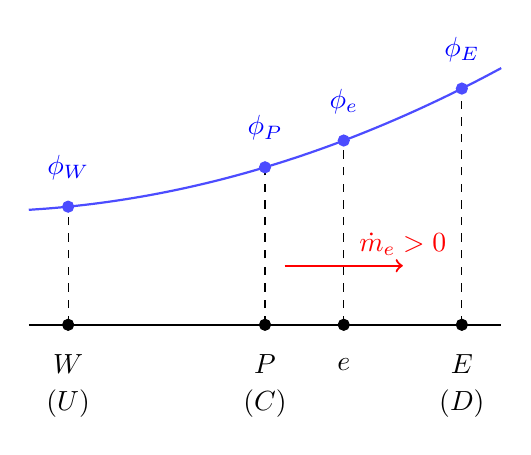
\begin{tikzpicture}
			% Points
			\def\zerox{0.5}
			\def\zeroy{1.5}
			\def\onex{3}
			\def\oney{2}
			\def\twox{5.5}
			\def\twoy{3}
			\def\coefa{1.5}
			\def\coefb{0.2}
			\def\coefc{0.04}
			% Ground
			\draw[thick] (0,0) -- ++(6,0);
			% Point W
			\filldraw[black] (\zerox,0) circle (2pt);
			\draw[dashed] (\zerox,0) -- ++(0,\zeroy);
			\node[black, yshift=-0.5cm] at (\zerox,0) {$W$};
			\node[black, yshift=-1cm] at (\zerox,0) {$(U)$};
			\filldraw[blue!70!white] (\zerox,\zeroy) circle (2pt);
			\node[blue, yshift=0.5cm] at (\zerox,\zeroy) {$\phi_W$};
			% Point P
			\filldraw[black] (\onex,0) circle (2pt);
			\draw[dashed] (\onex,0) -- ++(0,\oney);
			\node[black, yshift=-0.5cm] at (\onex,0) {$P$};
			\node[black, yshift=-1cm] at (\onex,0) {$(C)$};
			\filldraw[blue!70!white] (\onex,\oney) circle (2pt);
			\node[blue, yshift=0.5cm] at (\onex,\oney) {$\phi_P$};
			% Point e
			\filldraw[black] ({\onex+1},0) circle (2pt);
			\draw[dashed] ({\onex+1},0) -- ++(0,2.34);
			\node[black, yshift=-0.5cm] at ({\onex+1},0) {$e$};
			\filldraw[blue!70!white] ({\onex+1},2.34) circle (2pt);
			\node[blue, yshift=0.5cm] at ({\onex+1},2.34) {$\phi_e$};
			% Point E
			\filldraw[black] (\twox,0) circle (2pt);
			\draw[dashed] (\twox,0) -- ++(0,\twoy);
			\node[black, yshift=-0.5cm] at (\twox,0) {$E$};
			\node[black, yshift=-1cm] at (\twox,0) {$(D)$};
			\filldraw[blue!70!white] (\twox,\twoy) circle (2pt);
			\node[blue, yshift=0.5cm] at (\twox,\twoy) {$\phi_E$}; 
			% Blue line
			\draw[scale=1, domain=0:6, smooth, variable=\x, blue!70!white, thick] plot ({\x}, {\coefa + \coefb*(\x-\zerox) + \coefc*(\x-\zerox)*(\x-\onex)});
			% Mass flow
			\draw[->, red, thick] (3.25,0.75) -- ++(1.5,0) node[above]{$\dot{m}_e > 0$};
		\end{tikzpicture}
		\captionsetup{width=0.9\textwidth}
		\caption{QUICK when $(\vb{v} \vdot \vb{n})_e > 0$.}
		\label{fig:quick_1}
	\end{minipage}%
	\begin{minipage}{.5\textwidth}
		\centering
		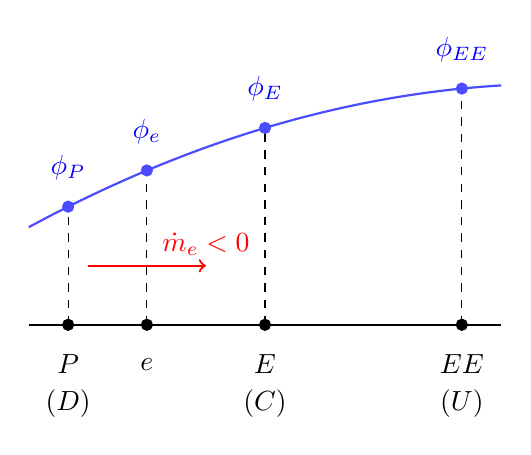
\begin{tikzpicture}
			% Points
			\def\zerox{0.5}
			\def\zeroy{1.5}
			\def\onex{3}
			\def\oney{2.5}
			\def\twox{5.5}
			\def\twoy{3}
			\def\coefa{1.5}
			\def\coefb{0.4}
			\def\coefc{-0.04}
			% Ground
			\draw[thick] (0,0) -- ++(6,0);
			% Point P
			\filldraw[black] (\zerox,0) circle (2pt);
			\draw[dashed] (\zerox,0) -- ++(0,\zeroy);
			\node[black, yshift=-0.5cm] at (\zerox,0) {$P$};
			\node[black, yshift=-1cm] at (\zerox,0) {$(D)$};
			\filldraw[blue!70!white] (\zerox,\zeroy) circle (2pt);
			\node[blue, yshift=0.5cm] at (\zerox,\zeroy) {$\phi_P$};
			% Point e
			\filldraw[black] ({\zerox+1},0) circle (2pt);
			\draw[dashed] ({\zerox+1},0) -- ++(0,1.96);
			\node[black, yshift=-0.5cm] at ({\zerox+1},0) {$e$};
			\filldraw[blue!70!white] ({\zerox+1},1.96) circle (2pt);
			\node[blue, yshift=0.5cm] at ({\zerox+1},1.96) {$\phi_e$};
			% Point e
			\filldraw[black] (\onex,0) circle (2pt);
			\draw[dashed] (\onex,0) -- ++(0,\oney);
			\node[black, yshift=-0.5cm] at (\onex,0) {$E$};
			\node[black, yshift=-1cm] at (\onex,0) {$(C)$};
			\filldraw[blue!70!white] (\onex,\oney) circle (2pt);
			\node[blue, yshift=0.5cm] at (\onex,\oney) {$\phi_E$}; 
			% Point ee
			\filldraw[black] (\twox,0) circle (2pt);
			\draw[dashed] (\twox,0) -- ++(0,\twoy);
			\node[black, yshift=-0.5cm] at (\twox,0) {$EE$};
			\node[black, yshift=-1cm] at (\twox,0) {$(U)$};
			\filldraw[blue!70!white] (\twox,\twoy) circle (2pt);
			\node[blue, yshift=0.5cm] at (\twox,\twoy) {$\phi_{EE}$}; 
			% Blue line
			\draw[scale=1, domain=0:6, smooth, variable=\x, blue!70!white, thick] plot ({\x}, {\coefa + \coefb*(\x-\zerox) + \coefc*(\x-\zerox)*(\x-\onex)});
			% Mass flow
			\draw[->, red, thick] (0.75,0.75) -- ++(1.5,0) node[above]{$\dot{m}_e < 0$};
		\end{tikzpicture}
		\captionsetup{width=0.9\textwidth}
		\caption{QUICK when $(\vb{v} \vdot \vb{n})_e < 0$.}
		\label{fig:quick_2}
	\end{minipage}
\end{figure}

\noindent
Let $(x_0, \phi_0)$, $(x_1, \phi_1)$, $(x_2, \phi_2)$ be the points which the polynomial $p(x)$ must interpolate, that is, $p(x_0) = \phi_0$, $p(x_1) = \phi_1$ and $p(x_2) = \phi_2$, satisfying $x_0 < x_1 < x_2$. If $(\vb{v} \vdot \vb{n})_e > 0$ then $x_0 = x_W$, $x_1 = x_P$ and $x_2 = x_E$, whereas $x_0 = x_P$, $x_1 = x_E$ and $x_2 = x_{EE}$ in case of $(\vb{v} \vdot \vb{n})_e < 0$. Let $p(x)$ be the following polynomial
\begin{equation}
	p(x) = a_0 + a_1 (x - x_0) + a_2 (x - x_0) (x - x_1), \quad a_0, a_1, a_2 \in \real
\end{equation}
Since the interpolating polynomial exists and is unique \colorbox{red}{referencia}, by imposing the interpolating condition, $p(x)$ will be the desired polynomial. The interpolating condition is,
\begin{equation}
	\left.
	\begin{aligned}
		p(x_0) &= a_0 = \phi_0 \\
		p(x_1) &= a_0 + a_1 (x_1 - x_0) = \phi_1 \\
		p(x_2) &= a_0 + a_1 (x_2 - x_0) + a_2 (x_2 - x_0) (x_2 - x_1) = \phi_2
	\end{aligned}	
	\right\}
\end{equation}
which yields the following linear system:
\begin{equation}
	\begin{pmatrix}
		1 & 0 & 0 \\
		1 & x_1 - x_0 & 0 \\
		1 & x_2 - x_0 & (x_2 - x_1)(x_2 - x_0)
	\end{pmatrix}
	\begin{pmatrix}
		a_0 \\ a_1 \\ a_2
	\end{pmatrix} = 
	\begin{pmatrix}
		\phi_0 \\ \phi_1 \\ \phi_2
	\end{pmatrix}
\end{equation}
The determinant of the system matrix is non-zero because the abscissae are distinct, therefore the solution is given by
\begin{equation}
	\left.
	\begin{aligned}
		a_0 &= \phi_0 \\
		a_1 &= \frac{\phi_1 - \phi_0}{x_1 - x_0} \\
		a_2 &= \frac{\phi_2 - \phi_0}{(x_2 - x_1)(x_2 - x_0)} - \frac{\phi_1 - \phi_0}{(x_2 - x_1)(x_1 - x_0)}
	\end{aligned}	
	\right\}
\end{equation}
and the polynomial is
\begin{equation} \label{eq:quick_polynomial_1}
	p(x) = 
	\phi_0 - 
	\frac{(x - x_2) (x - x_0)}{(x_2 - x_1)(x_1 - x_0)} (\phi_1 - \phi_0) + 
	\frac{(x - x_1)(x - x_0)}{(x_2 - x_1)(x_2 - x_0)} (\phi_2 - \phi_0)
\end{equation}
Assuming a uniform grid, \ie $x_1 - x_0 = x_2 - x_1 = L$ and the face $f$ located at the midpoint between nodal points, the approximation of $\phi_e$ given by QUICK scheme is
\begin{equation}
	\phi_e = -\frac{1}{8} \phi_0 + \frac{6}{8} \phi_1 + \frac{3}{8} \phi_2
\end{equation}
and depending on the sign of $(\vb{v} \vdot \vb{n})_e$,
\begin{equation} \label{eq:quick_approximation}
	\phi_e = 
	\left\{
	\begin{aligned}
		&-\frac{1}{8} \phi_U + \frac{6}{8} \phi_C + \frac{3}{8} \phi_D & 
		&\text{if} \quad (\vb{v} \vdot \vb{n})_e > 0 \\
		&-\frac{1}{8} \phi_D + \frac{6}{8} \phi_C + \frac{3}{8} \phi_U & 
		&\text{if} \quad (\vb{v} \vdot \vb{n})_e < 0 \\
	\end{aligned}
	\right.
\end{equation}
The output \eqref{eq:quick_approximation} provided by QUICK scheme is second--order accurate.


\subsubsection{Exponential--Difference Scheme (EDS)}

The exponential difference scheme assumes a distribution for $\phi$ based on the steady 2--dimensional generalized convection--diffusion equation with no source term, that is to say,
\begin{equation}
	\frac{\dd}{\dd{x}} (\rho u \phi) = \frac{\dd}{\dd{x}} \left( \Gamma \frac{\dd{\phi}}{\dd{x}} \right)
\end{equation}
where $u$ is the component of $\vb{v}$ in the $x$ direction. So as to ease the study, $\rho u$ and $\Gamma$ are assumed to be constant. Thereby the initial value problem obtained is
\begin{equation} \label{eq:eds_ivp}
	\left\{
	\begin{aligned}
		&\frac{\dd^2 \phi}{\phi{x^2}} - \frac{\rho u}{\Gamma} \frac{\dd{\phi}}{\dd{x}} = 0 & &\text{in } (x_P, x_E) \\
		&\phi(x_P) = \phi_P \\
		&\phi(x_E) = \phi_E \\
	\end{aligned}
	\right.
\end{equation}
Since \eqref{eq:eds_ivp} is a second order linear ODE with two boundary conditions, its solutions exists, is unique, and is given by
\begin{equation} \label{eq:eds_ivp_solution_1}
	\phi(x) = 
	\phi_P - 
	\frac{\phi_E - \phi_P}{e^{\frac{\rho u}{\Gamma} d_{PE}} - 1} + 
	\frac{\phi_E - \phi_P}{e^{\frac{\rho u}{\Gamma} d_{PE}} - 1} e^{\frac{\rho u}{\Gamma} (x - x_P)}
\end{equation}
Péclet's number for heat transfer is defined as the following ratio,
\begin{equation}
	\mathrm{Pe} = 
	\frac{\text{convection transport}}{\text{heat transport}} = 
	\frac{\rho u L}{\lambda / c_p}
\end{equation}
where $L$ is a characteristic length of the problem. Since $\lambda / c_p$ is the diffusion coefficient in equation \eqref{eq:cde_energy_equation}, it can be substituted by the diffusion coefficient $\Gamma$ of the generalized convection--diffusion equation, providing a new definition for Péclet's number 
\begin{equation}
	\mathrm{Pe} = 
	\frac{\rho u L}{\Gamma}
\end{equation}
Taking $d_{PE}$ as characteristic length and evaluating \eqref{eq:eds_ivp_solution_1} at $x = x_e$, the approximation of $\phi_e$ given by EDS in terms of Péclet's number is written as
\begin{equation}
	\frac{\phi_e - \phi_P}{\phi_E - \phi_P} =
	\frac{e^{\mathrm{Pe} \frac{d_{Pe}}{d_{PE}}} - 1}{e^{\mathrm{Pe}} - 1} 
\end{equation}


\subsubsection{Normalization of variables}

Owing to numerical reasons, it is convenient to normalize spatial and convective variables, that is to say, define new variables which take a rather small range of values. This is accomplished using the $DCU$ notation and defining 
\begin{align*}
	\hat{x} &= \frac{x - x_U}{x_D - x_U} \\
	\hat{\phi} &= \frac{\phi - \phi_U}{\phi_D - \phi_U}
\end{align*}
Of course, $(\hat{x}_U, \hat{\phi}_U) = (0,0)$, $(\hat{x}_D, \hat{\phi}_D) = (1,1)$ and $\hat{x}_C, \hat{x}_f \in (0,1)$. However, $\hat{\phi}$ is not necessarily in $[0,1]$ for all $x \in [0,1]$, nor does it have to be an increasing function. These situations are represented in figures \ref{fig:normalization_of_variables_1} and \ref{fig:normalization_of_variables_2}.

The normalized variable $\hat{\phi}_f$ can be computed directly as shown in section \colorbox{red}{referencia sección posterior} and, based on this, the variable at face,
\begin{equation}
	\phi_f = \phi_U + \hat{\phi}_f (\phi_D - \phi_U)
\end{equation}

\begin{figure}[h]
	\centering
	\begin{minipage}{.5\textwidth}
		\centering
		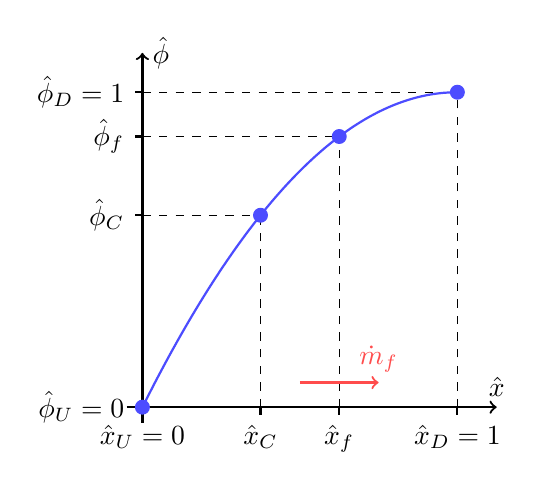
\begin{tikzpicture}
			\draw[->, thick] (0,-0.2) -- (0,4.5) node[right]{$\hat{\phi}$};
			\draw[->, thick] (-0.2,0) -- (4.5,0) node[above]{$\hat{x}$};
			\def\coefa{4}
			% x-U lines
			\draw[thick] (0,0) -- ++(0,-0.1) node[below]{$\hat{x}_U = 0$};
			% phi-U lines
			\draw[thick] (0,0) -- ++(-0.1,0) node[left]{$\hat{\phi}_U = 0$};
			% x-D lines
			\draw[thick] (4,0) -- ++(0,-0.1) node[below]{$\hat{x}_D = 1$};
			\draw[dashed] (4,0) -- ++(0,4);
			% phi-D lines
			\draw[thick] (0,\coefa) -- ++(-0.1,0) node[left]{$\hat{\phi}_D = 1$};
			\draw[dashed] (0,4) -- (4,4);
			% x-D lines
			\draw[thick] (1.5,0) -- ++(0,-0.1) node[below]{$\hat{x}_C$};
			\draw[dashed] (1.5,0) -- ++(0,{39/16});
			% phi-D lines
			\draw[thick] (0,{39/16}) -- ++(-0.1,0) node[left]{$\hat{\phi}_C$};
			\draw[dashed] (0,{39/16}) -- ++(1.5,0);
			% x-f lines
			\draw[thick] (2.5,0) -- ++(0,-0.1) node[below]{$\hat{x}_f$};
			\draw[dashed] (2.5,0) -- ++(0,{55/16});
			% phi-f lines
			\draw[thick] (0,{55/16}) -- ++(-0.1,0) node[left]{$\hat{\phi}_f$};
			\draw[dashed] (0,{55/16}) -- ++(2.5,0);
			% Mass flow
			\draw[->, red!70!white, thick] (2,.3125) -- ++(1,0) node[above]{$\dot{m}_f$};
			% Points
			\draw[scale=1, domain=0:4, smooth, variable=\x, blue!70!white, thick] plot ({\x}, {(-\x*(\x-2*\coefa))/\coefa});
			\filldraw[blue!70!white] (0,0) circle (2.5pt);
			\filldraw[blue!70!white] (4,4) circle (2.5pt);
			\filldraw[blue!70!white] (1.5,{39/16}) circle (2.5pt);
			\filldraw[blue!70!white] (2.5,{55/16}) circle (2.5pt);
		\end{tikzpicture}
		\captionsetup{width=0.9\textwidth}
		\caption{Scheme of normalized variables when $\hat{\phi}(x)$ is a strictly increasing function.}
		\label{fig:normalization_of_variables_1}
	\end{minipage}%
	\begin{minipage}{.5\textwidth}
		\centering
		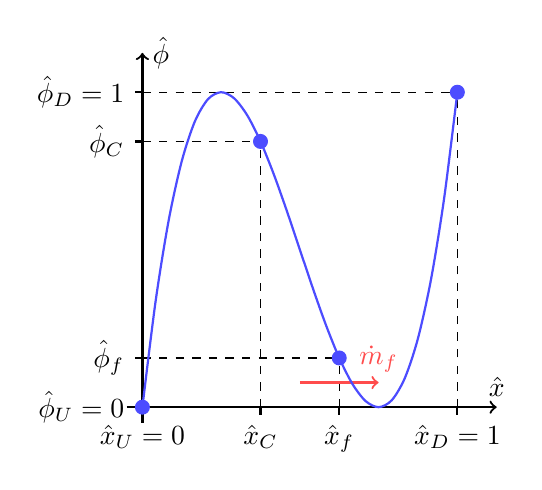
\begin{tikzpicture}
			\draw[->, thick] (0,-0.2) -- (0,4.5) node[right]{$\hat{\phi}$};
			\draw[->, thick] (-0.2,0) -- (4.5,0) node[above]{$\hat{x}$};
			\def\coefa{1}
			\def\coefb{-6}
			\def\coefc{9}
			% U lines
			\draw[thick] (0,0) -- ++(0,-0.1) node[below]{$\hat{x}_U = 0$};
			\draw[thick] (0,0) -- ++(-0.1,0) node[left]{$\hat{\phi}_U = 0$};
			% x-D lines
			\draw[thick] (4,0) -- ++(0,-0.1) node[below]{$\hat{x}_D = 1$};
			\draw[dashed] (4,0) -- (4,4);
			% phi-D lines
			\draw[thick] (0,4) -- ++(-0.1,0) node[left]{$\hat{\phi}_D = 1$};
			\draw[dashed] (0,4) -- (4,4);
			% x-C lines
			\draw[thick] (1.5,0) -- ++(0,-0.1) node[below]{$\hat{x}_C$};
			\draw[dashed] (1.5,0) -- ++(0,3.375);
			% phi-C lines
			\draw[thick] (0,3.375) -- ++(-0.1,0) node[left]{$\hat{\phi}_C$};
			\draw[dashed] (0,3.375) -- ++(1.5,0);
			% x-f lines
			\draw[thick] (2.5,0) -- ++(0,-0.1) node[below]{$\hat{x}_f$};
			\draw[dashed] (2.5,0) -- ++(0,0.625);
			% phi-f lines
			\draw[thick] (0,0.625) -- ++(-0.1,0) node[left]{$\hat{\phi}_f$};
			\draw[dashed] (0,0.625) -- ++(2.5,0);
			% Mass flow
			\draw[->, red!70!white, thick] (2,0.3125) -- ++(1,0) node[above]{$\dot{m}_f$};
			% Function
			\draw[scale=1, domain=0:4, smooth, variable=\x, blue!70!white, thick] plot ({\x}, {\coefa*\x^3 + \coefb*\x^2 + \coefc*\x});
			% Points
			\filldraw[blue!70!white] (0,0) circle (2.5pt);
			\filldraw[blue!70!white] (4,4) circle (2.5pt);
			\filldraw[blue!70!white] (1.5,3.375) circle (2.5pt);
			\filldraw[blue!70!white] (2.5,0.625) circle (2.5pt);
		\end{tikzpicture}
		\captionsetup{width=0.9\textwidth}
		\caption{Scheme of normalized variables when $\hat{\phi}(x)$ is not a strictly increasing function.}
		\label{fig:normalization_of_variables_2}
	\end{minipage}
\end{figure}

\subsubsection{High--order bounded convection schemes and SMART scheme}

As aforementioned, schemes whose order is higher than one might be unstable, producing oscillatory outputs for the convective variables. For instance, CDS, SUDS and QUICK are not bounded schemes. The conditions for stability and accuracy are formulated in \cite{gaskell1988curvature}:
\begin{enumerate}[label=(\roman*),topsep=0pt]
	\item $\hat{\phi}_f$ must be a continuous function of $\hat{\phi}_C$. \label{item:stability_accuracy_conditions_scheme_1}
	\item If $\hat{\phi}_C = 0$, then $\hat{\phi}_f = 0$.
	\item If $\hat{\phi}_C = 1$, then $\hat{\phi}_f = 1$.
	\item If $0 < \hat{\phi}_f < 1$, then $\hat{\phi}_C < \hat{\phi}_f < 1$.\label{item:stability_accuracy_conditions_scheme_2}
\end{enumerate}
Conditions \ref{item:stability_accuracy_conditions_scheme_1} through \ref{item:stability_accuracy_conditions_scheme_2} are represented in figure \ref{fig:stability_accuracy_conditions_scheme}. A bounded convective scheme must output results lying within the shadowed region.

\begin{figure}[h]
	\centering
	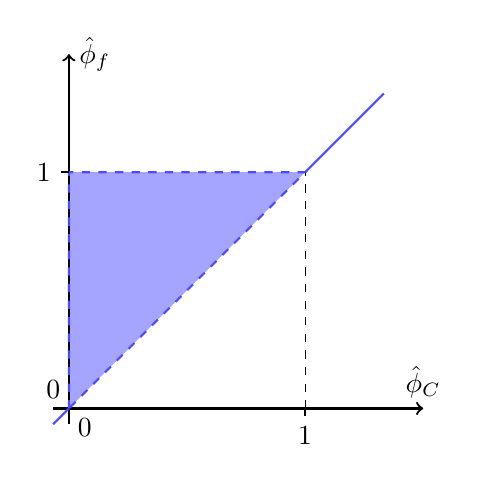
\begin{tikzpicture}
		% Filled zone
		\fill[fill=blue!70!white, opacity=0.5] (0,0) -- (3,3) -- (0,3) -- cycle;
		% Axis
		\draw[->, thick] (-0.2,0) -- (4.5,0) node[above]{$\hat{\phi}_C$};
		\draw[->, thick] (0,-0.2) -- (0,4.5) node[right]{$\hat{\phi}_f$};
		% Countour of filled zine
		\draw[blue!70!white, thick, dashed] (0,0) -- ++(0,3) -- ++(3,0) -- cycle;
		% Marks
		\node[below,xshift=2mm] at (0,0) {$0$};
		\node[above,xshift=-2mm] at (0,0) {$0$};
		\draw[thick] (3,0) -- ++(0,-0.1) node[below]{$1$};
		\draw[thick] (0,3) -- ++(-0.1,0) node[left]{$1$};
		\draw[dashed] (3,0) -- ++(0,3);
		% Function
		\draw[scale=1, domain=-0.2:0, smooth, variable=\x, blue!70!white, thick] plot ({\x}, {\x});
		\draw[scale=1, domain=3:4, smooth, variable=\x, blue!70!white, thick] plot ({\x}, {\x});
	\end{tikzpicture}
	\captionsetup{width=0.5\textwidth}
	\caption{High--order bounded convection schemes conditions for stability.}
	\label{fig:stability_accuracy_conditions_scheme}
\end{figure}

The SMART scheme (Sharp and Monotonic Algorithm for Realistic Transport) is a bounded convective scheme \cite{gaskell1988curvature}, given by:
\begin{equation}
	\hat{\phi}_f = 
	\left\{
	\begin{aligned}
		&-\frac{\hat{x}_f (1 - 3 \hat{x}_C + 2 \hat{x}_f)}{\hat{x}_C (\hat{x}_C - 1)} \hat{\phi}_C & 
		&\text{if} \quad 0 < \hat{\phi}_C < \frac{\hat{x}_C}{3} \\
		&\frac{\hat{x}_f (\hat{x}_f - \hat{x}_C)}{1 - \hat{x}_C} + \frac{\hat{x}_f (\hat{x}_f - 1)}{\hat{x}_C (\hat{x}_C - 1)} \hat{\phi}_C &
		&\text{if} \quad \frac{\hat{x}_C}{3} < \hat{\phi}_C <  \frac{\hat{x}_C (1 + \hat{x}_f - \hat{x}_C)}{\hat{x}_f} \\
		&1 & &\text{if} \quad \frac{\hat{x}_C (1 + \hat{x}_f - \hat{x}_C)}{\hat{x}_f} < \hat{\phi_C} < 1 \\
		&\hat{\phi}_C & &\text{otherwise} \\
	\end{aligned}
	\right.
\end{equation}

\subsubsection{Summary of schemes}

Below a summary of the studied schemes is shown:

\begin{table}[h]
	\centering
	\begin{tabular}{ll}
		\toprule[0.50mm]
		\textbf{Scheme} & \textbf{Face value} \\
		\midrule[0.25mm]
		
		\bottomrule[0.50mm]
	\end{tabular}
\end{table}